\section{Example for EnergyPlus Line Diagram Generation}\label{example-for-energyplus-line-diagram-generation}

A series of figures are provided below to detail the process for generating an EnergyPlus line diagram.

1.~~~~\textbf{Obtain a simple engineering line diagram for the system.} This system is a simple cooling system that employs a primary/secondary pumping setup with a one-way common pipe to circulate chilled water through a building. Figure~\ref{fig:simple-line-diagram-for-the-example-system} shows the simple line diagram for the system.

\begin{figure}[hbtp] % fig 3
\centering
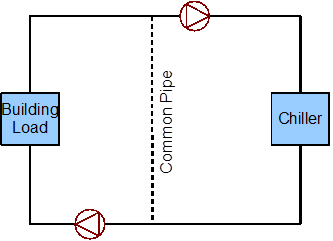
\includegraphics[width=0.9\textwidth, height=0.9\textheight, keepaspectratio=true]{media/image003.png}
\caption{Simple line diagram for the example system, (recreated from Reed and Davis 2007) \protect \label{fig:simple-line-diagram-for-the-example-system}}
\end{figure}

2.~~~~\textbf{Identify all the loops in the system.} This system contains only one plant loop. Loop name: Cooling Loop.

\textbf{3.~~~~Identify the demand side and supply side of the loop.} ~The half loops are depicted in Figure~\ref{fig:breakdown-of-a-loop-into-its-constituent-half}.

\begin{figure}[hbtp] % fig 4
\centering
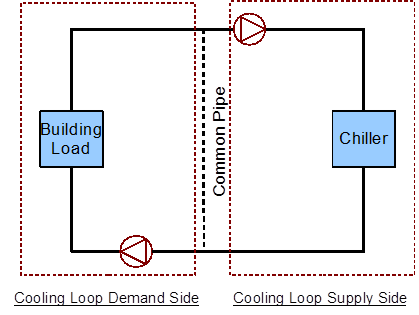
\includegraphics[width=0.9\textwidth, height=0.9\textheight, keepaspectratio=true]{media/image004.png}
\caption{Breakdown of a loop into its constituent half-loops \protect \label{fig:breakdown-of-a-loop-into-its-constituent-half}}
\end{figure}

4.~~~~\textbf{Identify the components in the system.} While identifying the main components in the loop, it should be noted that this loop has a primary/secondary pumping setup, and that there is a common pipe that allows for flow imbalance. (Note: The \emph{PlantLoop} object in EnergyPlus has a provision for the input of a common pipe. The user only has to specify the existence of a common pipe in the loop, and the program calculates its position in the loop). The primary pump is shown below is shown in Figure~\ref{fig:a-component-in-the-loop}.

\begin{figure}[hbtp] % fig 5
\centering
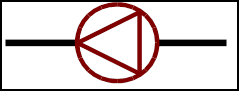
\includegraphics[width=0.9\textwidth, height=0.9\textheight, keepaspectratio=true]{media/image005.png}
\caption{A component in the loop \protect \label{fig:a-component-in-the-loop}}
\end{figure}

5.~~~~\textbf{Identify all the nodes in the system.} As mentioned above, placing a node on each side of a component is a good way to pinpoint all the nodes in the system. This process should be repeated for every component in the loop. Figure~\ref{fig:node-placement-on-components} shows the placement of all the nodes on Individual components, while Figure~\ref{fig:nodes-in-the-system} shows all the nodes in the system.

\begin{figure}[hbtp] % fig 6
\centering
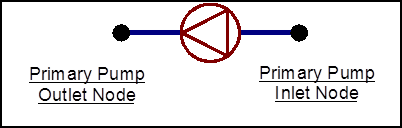
\includegraphics[width=0.9\textwidth, height=0.9\textheight, keepaspectratio=true]{media/image006.png}
\caption{Node placement on components \protect \label{fig:node-placement-on-components}}
\end{figure}

\begin{figure}[hbtp] % fig 7
\centering
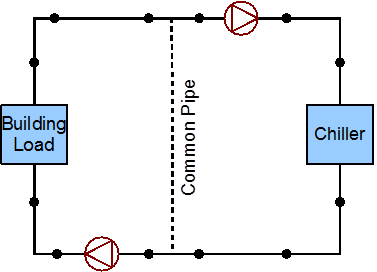
\includegraphics[width=0.9\textwidth, height=0.9\textheight, keepaspectratio=true]{media/image007.png}
\caption{Nodes in the system \protect \label{fig:nodes-in-the-system}}
\end{figure}

Note: No nodes were placed on the common pipe, but its existence should be specified in the \emph{PlantLoop} object.

6.~~~~\textbf{Identify all the branches in the system.} Remember to add the bypass branches to the operating components (except the pumps). Branches have to start and end with nodes, and should contain at least one component. The branches are denoted by the blue lines in Figure~\ref{fig:branch-definition}.

\begin{figure}[hbtp] % fig 8
\centering
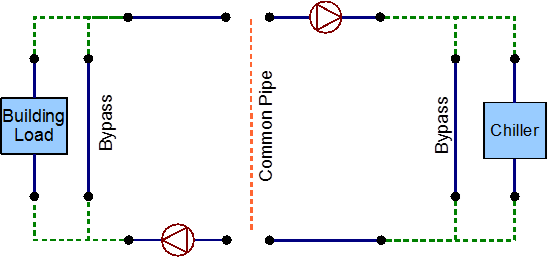
\includegraphics[width=0.9\textwidth, height=0.9\textheight, keepaspectratio=true]{media/image008.png}
\caption{Branch definition \protect \label{fig:branch-definition}}
\end{figure}

7.~~~~\textbf{Identify the position of the connectors in the system.} The \emph{PlantLoop} accepts only one splitter-mixer pair per half loop. The connectors are defined by using branches; a splitter can have one inlet branch and any number of outlet branches whereas a mixer can have any number of inlet branches and one outlet branch. All the connectors in the loop are denoted by the green lines in Figure~\ref{fig:splitters-and-mixers-in-the-loop}.

\begin{figure}[hbtp] % fig 9
\centering

\includegraphics[width=0.9\textwidth, height=0.9\textheight, keepaspectratio=true]{media/image009.png}
\caption{Splitters and mixers in the loop \protect \label{fig:splitters-and-mixers-in-the-loop}}
\end{figure}

8.~~~~An EnergyPlus diagram can be generated by using all the identified components. The complete schematic is shown in Figure~\ref{fig:complete-energyplus-line-diagram}.

\begin{figure}[hbtp] % fig 10
\centering
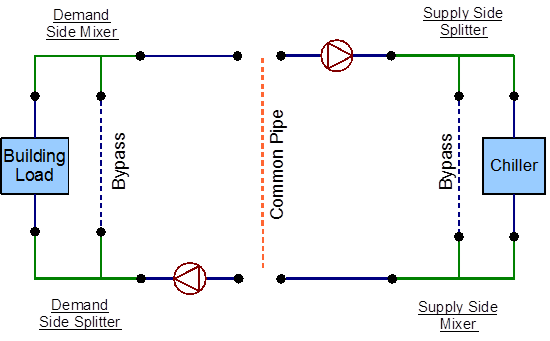
\includegraphics[width=0.9\textwidth, height=0.9\textheight, keepaspectratio=true]{media/image010.png}
\caption{Complete EnergyPlus line diagram \protect \label{fig:complete-energyplus-line-diagram}}
\end{figure}
